\documentclass[border=4pt]{standalone}
\usepackage{amsmath}
\usepackage{tikz}
\usetikzlibrary{arrows.meta}

% Esquema del criterio de la primera derivada.
% #1 = desplazamiento, #2 = etiqueta del panel, #3 = curva (en coordenadas locales,
% a = 1, p = 2, b = 3), #4 = signo a la izquierda, #5 = signo a la derecha
\newcommand{\panel}[5]{%
  \begin{scope}[shift={#1}]
    \draw[gray!70] (-0.2,0) -- (4.2,0);
    \draw[line width=1pt, black!75] #3;
    \foreach \x/\l in {1/a,2/p,3/b} {
      \fill (\x,0) circle (1.2pt);
      \node[below=2pt, font=\scriptsize] at (\x,0) {$\l$};
    }
    \draw[-{Latex[length=3pt]}] (0.8,-0.55) -- (1.35,-0.55) -- (1.45,-0.3);
    \draw[-{Latex[length=3pt]}] (3.2,-0.55) -- (2.65,-0.55) -- (2.55,-0.3);
    \node[anchor=east, font=\scriptsize] at (0.75,-0.55) {$f'#4 0$};
    \node[anchor=west, font=\scriptsize] at (3.25,-0.55) {$f'#5 0$};
    \node[font=\small] at (2,-1.25) {#2};
  \end{scope}}

\begin{document}
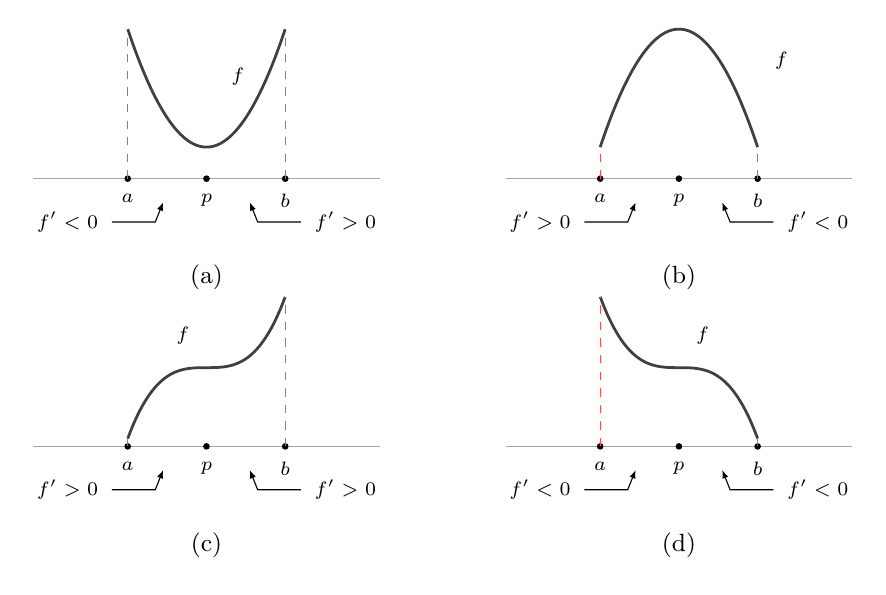
\begin{tikzpicture}[x=1cm, y=1cm]
    \panel{(0,0)}{(a)}{plot[domain=1:3, smooth, samples=40] (\x,{0.4+1.5*(\x-2)^2})}{<}{>}
    \draw[red!70, dashed] (1,0) -- (1,1.9); \draw[red!70, dashed] (3,0) -- (3,1.9);
    \node[font=\scriptsize] at (2.4,1.3) {$f$};
    \panel{(6,0)}{(b)}{plot[domain=1:3, smooth, samples=40] (\x,{1.9-1.5*(\x-2)^2})}{>}{<}
    \draw[red!70, dashed] (7,0) -- (7,0.4); \draw[red!70, dashed] (9,0) -- (9,0.4);
    \node[font=\scriptsize] at (9.3,1.5) {$f$};
    \panel{(0,-3.4)}{(c)}{plot[domain=1:3, smooth, samples=40] (\x,{1+0.9*(\x-2)^3})}{>}{>}
    \draw[red!70, dashed] (1,-3.4) -- (1,-3.3); \draw[red!70, dashed] (3,-3.4) -- (3,-1.5);
    \node[font=\scriptsize] at (1.7,-2) {$f$};
    \panel{(6,-3.4)}{(d)}{plot[domain=1:3, smooth, samples=40] (\x,{1-0.9*(\x-2)^3})}{<}{<}
    \draw[red!70, dashed] (7,-3.4) -- (7,-1.5); \draw[red!70, dashed] (9,-3.4) -- (9,-3.3);
    \node[font=\scriptsize] at (8.3,-2) {$f$};
\end{tikzpicture}
\end{document}
